\documentclass[11pt]{article}

\usepackage[margin=1in]{geometry}
\usepackage{amsmath,amssymb,amsthm,mathtools,bm}
\usepackage{booktabs,longtable,array,multirow,tabularx}
\usepackage{enumitem}
\usepackage{xcolor}
\usepackage{hyperref}
\usepackage{microtype}
\usepackage{caption}
\usepackage{subcaption}
\usepackage{placeins}
\usepackage{graphicx}
\usepackage{tikz}
\usetikzlibrary{arrows.meta,positioning,calc,fit,shapes.geometric}

\hypersetup{colorlinks=true,linkcolor=blue!50!black,citecolor=blue!50!black,urlcolor=blue!50!black}

\newtheorem{theorem}{Theorem}[section]
\newtheorem{proposition}[theorem]{Proposition}
\newtheorem{lemma}[theorem]{Lemma}
\newtheorem{corollary}[theorem]{Corollary}
\newtheorem{assumption}[theorem]{Assumption}
\theoremstyle{definition}
\newtheorem{definition}[theorem]{Definition}
\theoremstyle{remark}
\newtheorem{remark}[theorem]{Remark}

\newcommand{\R}{\mathbb{R}}
\newcommand{\one}{\mathbf{1}}
\newcommand{\diag}{\operatorname{diag}}
\newcommand{\argmin}{\operatorname*{arg\,min}}
\newcommand{\E}{\mathbb{E}}
\newcommand{\Var}{\operatorname{Var}}
\newcommand{\Cov}{\operatorname{Cov}}
\newcommand{\Tr}{\operatorname{Tr}}
\newcommand{\calF}{\mathcal{F}}
\newcommand{\calE}{\mathcal{E}}
\newcommand{\calL}{\mathcal{L}}
\newcommand{\T}{^{\mathsf T}}
\newcommand{\SD}{S_D}

\title{Adaptive Green Risk Fields for Causal Fraud Detection}
\author{Maksim Kosmakov\thanks{University of Cincinnati. Email: \texttt{maximkosmakov@gmail.com}.}}
\date{}

\begin{document}
\maketitle

\begin{abstract}
Fraud screening on transaction streams is a delayed-feedback graph problem: a deployable score must be computed before the candidate transaction, and before any label from that transaction can influence the system. We introduce an adaptive Green risk field that propagates released fraud history over a dynamic transaction graph while weighting each node by the reliability of its local history. The estimator is a graph-Tikhonov minimizer, an implicit message-passing layer, and the posterior mean of a Gaussian Markov random field. Its MSE decomposition separates variance reduction from graph-induced bias, yielding a regime criterion: smoothing is most useful when local histories are sparse or noisy and least useful when released history is already high-confidence. In block-causal experiments on IEEE-CIS, tail-ranking models using Green-risk features improve over raw released history across all tested label-release delays. The standalone graph marginal is positive under immediate release and attenuates as labels are delayed, consistent with the regime criterion. Leakage audits, label-permutation placebo tests, paired block-bootstrap intervals, calibration diagnostics, posterior-uncertainty checks, and an Elliptic++ high-confidence regime check are consistent with this regime account. The resulting layer is interpretable, temporally auditable, and directly applicable to fraud alert ranking under delayed labels.
\end{abstract}

\noindent\textbf{Keywords:} fraud detection; dynamic graphs; causal machine learning; graph Laplacian; label propagation; risk ranking; delayed labels

\vspace{0.75em}

\section{Introduction and positioning}

Fraud detection is usually evaluated as supervised classification, whereas deployment is chronological decision support. A production score may use only the graph state, transaction history, and labels available before the candidate transaction is evaluated. This chronological constraint is substantive: fraud risk is carried by identifiers that recur across time--cards, devices, email domains, addresses, accounts, merchants, and wallets--while labels are delayed and timestamps may be tied. A graph-risk layer therefore has to combine relational evidence, timestamp-level measurability, and transparent alert-ranking features.

The construction starts from released history. For each entity $v$, let $H_v$ summarize the fraud rate among labels released before scoring. This local estimate is reliable for heavily observed endpoints and unstable for new or thinly observed endpoints. The adaptive Green field
\begin{equation}
        S_D=(L+D)^{-1}DH,
        \label{eq:main-field}
\end{equation}
uses the historical graph Laplacian $L$ to propagate evidence from neighboring entities and a diagonal confidence matrix $D=\diag(d_v)$ to control the weight assigned to $H_v$. Large $d_v$ anchors the estimate near $H_v$; small $d_v$ permits more graph propagation.

This construction uses standard graph-regularization tools in a delayed-label fraud-ranking protocol. Graph-based semi-supervised learning and label propagation use Laplacian energies to extend sparse labels over weighted graphs \cite{zhu2003,zhou2004,belkin2006,smola2003,chapelle2006}. Gaussian Markov random fields, spectral graph theory, and graph signal processing provide the language of graph-smooth priors, precision matrices, Green operators, and posterior covariance \cite{rueheld,chung1997,rasmussen2006,shuman2013,ortega2018}. Fraud and anomaly detection add the operational constraints of imbalance, delayed feedback, and fixed alert budgets \cite{boltonhand2002,phua2010,davis2006relationship,saito2015precision}, while graph anomaly detection and dynamic-network learning motivate relational modeling under evolving structure \cite{akoglu2015,ranshous2015,weber2019,elmougy2023,kipf2017,hamilton2017,velickovic2018,pareja2020,sankar2020,xu2020,rossi2020}. This paper studies an auditable released-history layer whose inputs, graph state, and label availability are fixed at each scoring time.

The theory identifies the estimator's operating regime. The field is a Laplacian energy minimizer, a convex averaging operator, a fixed point of an implicit message-passing rule, and a Gaussian Markov random field posterior mean. Its MSE decomposition separates the variance reduction obtained by smoothing noisy histories from the bias introduced when graph neighborhoods mix different risks. The method is therefore tied to a concrete bias--variance regime: smoothing is useful only when variance reduction exceeds graph-induced bias. Calibration is reported separately from tail ranking, since top-alert ranking scores and calibrated probabilities serve different operational targets \cite{zadrozny2002,niculescu2005,guo2017}.

The experiments are organized around this regime boundary. On IEEE-CIS, many graph endpoints have sparse or noisy released histories. The Green field supplies a positive standalone marginal under immediate release; validation-selected tail-ranking models using Green-risk features remain positive across all tested release delays. On Elliptic++, released address history is already strong at the top alert budget, leaving little residual signal for exact local smoothing. The datasets therefore play different roles: IEEE-CIS supplies evidence for graph-based alert ranking in a sparse-history regime, and Elliptic++ checks the high-confidence regime predicted by the theory.

The paper contributes a timestamp-causal released-history construction for dynamic fraud graphs, an adaptive Green field with variational, maximum-principle, message-passing, and GMRF interpretations, an MSE-based regime criterion for graph smoothing, and a block-causal empirical protocol with graph-vs-history ablations, delay sweeps, leakage audits, placebo tests, bootstrap intervals, calibration diagnostics, and posterior-uncertainty checks.

\section{Causal transaction graph}
\label{sec:causal-setting}

Let transactions arrive in chronological order. Before a candidate transaction $x_t$ is scored, the available information is
\[
    \calF_{t^-}=\sigma\{\text{transactions before }t,\ \text{edges inserted before }t,\ \text{labels released before }t\}.
\]
Every feature used by the score must be $\calF_{t^-}$-measurable. For each relation type $r$ we form a weighted historical graph
\[
    G_{t^-}^{(r)}=(V_{t^-},E_{t^-}^{(r)},W_{t^-}^{(r)}),
\]
whose nodes are reusable transaction entities and whose edges encode causal co-occurrence, frequency, recency, or relation strength. The corresponding combinatorial Laplacian is
\[
    L_{t^-}^{(r)}=D_{W,t^-}^{(r)}-W_{t^-}^{(r)},
\]
and relation layers may be combined as
\begin{equation}
    L_{t^-}=\sum_r \theta_r L_{t^-}^{(r)},\qquad \theta_r\ge 0.
    \label{eq:relation-layers}
\end{equation}
Candidate edges are withheld until after scoring. If a new entity appears in the candidate transaction, it is temporarily added as an isolated node so that endpoint features are defined without using the candidate edge itself.

\begin{figure}[t]
\centering
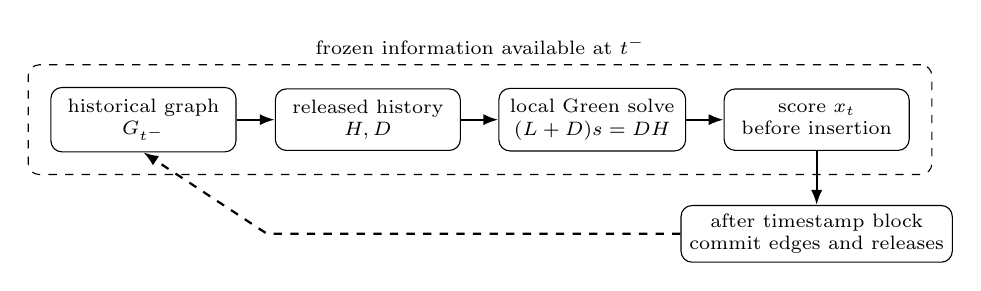
\begin{tikzpicture}[
    font=\scriptsize,
    block/.style={draw,rounded corners,align=center,minimum width=2.35cm,minimum height=0.78cm,inner sep=4pt},
    smallblock/.style={draw,rounded corners,align=center,minimum width=2.35cm,minimum height=0.72cm,inner sep=3pt},
    arrow/.style={-{Latex[length=1.9mm]},thick}
]
\node[block] (past) at (0,0) {historical graph\\$G_{t^-}$};
\node[block] (hist) at (2.85,0) {released history\\$H,D$};
\node[block] (solve) at (5.70,0) {local Green solve\\$(L+D)s=DH$};
\node[block] (score) at (8.55,0) {score $x_t$\\before insertion};
\node[smallblock] (commit) at (8.55,-1.45) {after timestamp block\\commit edges and releases};
\draw[arrow] (past) -- (hist);
\draw[arrow] (hist) -- (solve);
\draw[arrow] (solve) -- (score);
\draw[arrow] (score) -- (commit);
\draw[arrow,dashed] (commit.west) -- ++(-5.25,0) -- (past.south);
\node[draw,dashed,rounded corners,fit=(past)(hist)(solve)(score),inner sep=8pt,label={[font=\scriptsize]above:{frozen information available at $t^-$}}] {};
\end{tikzpicture}
\caption{Timestamp-block causal scoring. All transactions with the same timestamp are scored against the same frozen historical state. Candidate edges and labels from that block are committed only after the block has been scored.}
\label{fig:graph}
\end{figure}

The released-history vector is built from labels whose release time precedes the scoring time. A convenient shrinkage estimate is
\begin{equation}
    H_v=\frac{f_v+\alpha \bar p}{n_v+\alpha},
    \label{eq:history}
\end{equation}
where $f_v$ and $n_v$ are released fraud and exposure counts for node $v$, and $\bar p$ is the causal global fraud rate. The confidence matrix
\[
    D=\diag(d_v),\qquad d_v>0,
\]
records the reliability assigned to each local history. The experiments use the concave rule $d_v=\alpha+\sqrt{n_v}$, so confidence grows with evidence without assigning overwhelming precision to high-degree hubs. A beta-binomial calculation below gives a formal precision scale and motivates the concave approximation.

\section{Adaptive Green smoothing}
\label{sec:theory}

For the theory, fix one causal graph snapshot and suppress time subscripts. The adaptive field is
\[
    \SD=(L+D)^{-1}DH.
\]
Its basic variational form explains the two forces in the estimator: graph smoothness and fidelity to released local history.

\begin{proposition}[Energy minimizer]
Let $L\succeq0$ be a graph Laplacian and $D\succ0$ diagonal. Then $\SD$ is the unique minimizer of
\begin{equation}
    \calE(s)=\frac12\sum_{(u,v)\in E}w_{uv}(s_u-s_v)^2
    +\frac12\sum_{v\in V}d_v(s_v-H_v)^2.
    \label{eq:energy}
\end{equation}
\end{proposition}

\begin{proof}
Since $s^\top Ls=\sum_{(u,v)}w_{uv}(s_u-s_v)^2$, the energy is
\[
    \calE(s)=\frac12s^\top Ls+\frac12(s-H)^\top D(s-H).
\]
The Hessian is $L+D\succ0$, so the minimizer is unique. Stationarity gives $(L+D)s=DH$, hence $s=(L+D)^{-1}DH$.
\end{proof}

The same linear system also gives a maximum principle. Define
\[
    P_D=(L+D)^{-1}D.
\]
Because $L\one=0$, we have $(L+D)\one=D\one$, and therefore $P_D\one=\one$. Since $L+D$ is an invertible symmetric M-matrix, $(L+D)^{-1}$ is entrywise nonnegative, so $P_D\ge0$ entrywise.

\begin{lemma}[Convex-combination operator]
Each component of $\SD=P_DH$ is a convex combination of the entries of $H$.
\end{lemma}

\begin{corollary}[Maximum principle and non-expansiveness]
If $m\le H_v\le M$ for all $v$, then
\[
    m\le (\SD)_v\le M\qquad \forall v.
\]
Moreover, for any histories $H,\widetilde H$,
\[
    \|P_DH-P_D\widetilde H\|_\infty\le \|H-\widetilde H\|_\infty.
\]
\end{corollary}

Operationally, smoothing cannot create risk scores outside the range of released histories, and perturbations of the released histories are not amplified in sup norm.

Writing $L=D_W-W$ turns the optimality equation into the nodewise fixed point
\begin{equation}
    (\SD)_v=\frac{d_vH_v+\sum_{u\sim v}w_{uv}(\SD)_u}{d_v+\sum_{u\sim v}w_{uv}}.
    \label{eq:nodewise}
\end{equation}
Thus $d_v$ acts as a trust parameter. When $d_v$ is large compared with the weighted degree of $v$, the score is anchored near $H_v$; when $d_v$ is small, the score moves toward a weighted neighborhood average. This gives an implicit message-passing layer with a closed-form linear solve.

Local computation follows from the same linear algebra. If $A=L+D$ and nodes are partitioned into a boundary/local set $B$ and an interior/far set $I$, then
\[
    A=\begin{pmatrix}A_{BB}&A_{BI}\\ A_{IB}&A_{II}\end{pmatrix},
    \qquad
    S_B=A_{BB}-A_{BI}A_{II}^{-1}A_{IB}.
\]
The boundary values of $s=A^{-1}DH$ satisfy
\[
    S_Bs_B=(DH)_B-A_{BI}A_{II}^{-1}(DH)_I.
\]
This identity motivates local Green computations. The implementation in this paper computes exact fields on bounded radius-2/cap-100 ego graphs, so the reported field is exact on the selected local graph.

The field also has a probabilistic interpretation. Consider the graph-smooth prior and heteroskedastic observation model
\[
    p(s)\propto \exp\left(-\frac12s^\top Ls\right),
    \qquad
    H_v\mid s_v\sim N(s_v,d_v^{-1})\quad\text{independently}.
\]

\begin{proposition}[GMRF posterior mean]
The posterior is Gaussian with
\[
    \E[s\mid H]=(L+D)^{-1}DH=\SD,
    \qquad
    \Cov(s\mid H)=(L+D)^{-1}.
\]
\end{proposition}

\begin{proof}
The negative log posterior is, up to constants,
\[
    \frac12s^\top Ls+\frac12(H-s)^\top D(H-s)
    =\frac12s^\top(L+D)s-s^\top DH+\text{const.}
\]
Completing the square gives precision $L+D$, covariance $(L+D)^{-1}$, and mean $(L+D)^{-1}DH$.
\end{proof}

The prior precision $L$ is singular, as in an intrinsic GMRF, but the posterior is proper because $D\succ0$. The posterior covariance gives a per-node uncertainty estimate
\begin{equation}
    \sigma_v^2=[(L+D)^{-1}]_{vv}.
    \label{eq:posterior-var}
\end{equation}
For a transaction with endpoints $a,b$, the corresponding diagnostic features include $\sigma_a,\sigma_b$ and standardized risk contrasts such as
\[
    \frac{(\SD)_a-\bar H}{\sigma_a},
    \qquad
    \frac{(\SD)_b-\bar H}{\sigma_b},
    \qquad
    \frac{(\SD)_a-(\SD)_b}{\sqrt{\sigma_a^2+\sigma_b^2}}.
\]

\begin{lemma}[Posterior variance bound]
For every node,
\[
    0<\sigma_v^2\le \frac1{d_v}.
\]
Equality holds for an isolated node.
\end{lemma}

\begin{proof}
Since $L\succeq0$, we have $L+D\succeq D\succ0$. By antitonicity of the inverse on positive definite matrices, $(L+D)^{-1}\preceq D^{-1}$. Taking diagonal entries gives the bound.
\end{proof}

A beta-binomial model suggests one possible scale for $D$. If $H_v$ is the posterior mean of a fraud rate with prior $\operatorname{Beta}(a,b)$ and $N_v$ released exposures,
\[
    H_v=\frac{a+F_v}{a+b+N_v},
\]
then the posterior variance is
\[
    \Var(p_v\mid\text{data})=\frac{H_v(1-H_v)}{a+b+N_v+1}.
\]
A variance-matched precision is therefore
\begin{equation}
    d_v^\star=\frac{a+b+N_v+1}{H_v(1-H_v)}.
    \label{eq:eb-d}
\end{equation}
Because fraud rates are small and $H_v(1-H_v)$ can be tiny, a capped precision is safer:
\begin{equation}
    d_v^{\mathrm{EB,cap}}=\min\left\{d_{\max},\frac{a+b+N_v+1}{\max\{H_v(1-H_v),\epsilon\}}\right\}.
    \label{eq:eb-cap}
\end{equation}
The square-root rule used in the final experiments is a conservative concave alternative: it lets confidence grow with evidence without letting hubs dominate the smoothing system.

\section{When does smoothing help?}
\label{sec:mse}

The next result gives the regime criterion. Suppose there is a latent risk vector $r\in\R^V$ and the released history satisfies
\[
    H=r+\eta,
    \qquad
    \E\eta=0,
    \qquad
    \Cov(\eta)=D^{-1}.
\]
The raw estimator is $H$ and the smoothed estimator is $P_DH$, where $P_D=(L+D)^{-1}D$. Smoothing changes the error in two directions: it reduces observation variance, but it biases the estimate toward graph-smooth vectors.

\begin{theorem}[MSE decomposition for adaptive Green smoothing]
\label{thm:mse-decomp}
Under the latent risk model above,
\begin{equation}
\begin{aligned}
    \operatorname{MSE}(P_DH)-\operatorname{MSE}(H)
    & = \|(L+D)^{-1}Lr\|_2^2 \\
    &\quad - \Tr\left[D^{-1}-(L+D)^{-1}D(L+D)^{-1}\right].
\end{aligned}
\label{eq:mse-decomp}
\end{equation}
The first term is graph-smoothing bias. The second term is estimator-variance reduction and is nonnegative.
\end{theorem}

\begin{proof}
The smoothed estimator has bias
\[
    \E[P_DH]-r=(P_D-I)r=-(L+D)^{-1}Lr.
\]
Its variance trace is
\[
    \Tr(P_DD^{-1}P_D^\top)=\Tr((L+D)^{-1}D(L+D)^{-1}).
\]
Subtracting the variance trace of $H$, namely $\Tr(D^{-1})$, gives \eqref{eq:mse-decomp}. The variance-reduction term is nonnegative because $0\preceq (L+D)^{-1}D(L+D)^{-1}\preceq D^{-1}$.
\end{proof}

The theorem gives the regime criterion used throughout the experiments. Graph smoothing is useful when histories are noisy enough for the variance term to matter and when true risk is sufficiently smooth along the chosen graph. Its marginal value decreases when raw released history is already high-confidence.

\begin{corollary}[High-confidence limit]
\label{cor:high-confidence}
Fix $L$ and $r$, and let $D_k\succ0$ satisfy $\lambda_{\min}(D_k)\to\infty$. Then
\[
    \Tr\left[D_k^{-1}-(L+D_k)^{-1}D_k(L+D_k)^{-1}\right]\to 0,
\]
and
\[
    \|(L+D_k)^{-1}Lr\|_2^2\to 0.
\]
Thus the available MSE gain from smoothing vanishes as raw-history confidence grows.
\end{corollary}

For ranking metrics such as AUC-PR or $P@1\%$, the corollary should be read as a regime guide. Sparse histories leave variance for smoothing to reduce; highly discriminative histories leave less residual signal, so smoothing can perturb an already accurate ranking unless graph neighborhoods are nearly bias-free.

\section{Scoring architecture}
\label{sec:architecture}

For a candidate transaction with endpoints $a,b$ and attributes $x$, the adaptive field produces endpoint features such as
\[
    (\SD)_a,
    \quad
    (\SD)_b,
    \quad
    (\SD)_a+(\SD)_b,
    \quad
    \max\{(\SD)_a,(\SD)_b\},
    \quad
    |(\SD)_a-(\SD)_b|.
\]
With posterior uncertainty, the feature family can be expanded by $\sigma_a,\sigma_b$ and standardized risk terms.

The supervised tabular models use LightGBM-style gradient-boosted trees \cite{ke2017lightgbm}. The baseline model is denoted
\[
    M3=T+C+G+P,
\]
where $T$ are transaction attributes, $C$ are cold-start/count/recency features, $G$ are graph-aggregate features, and $P$ are temporal-link history features. The selected alert-ranking model adds adaptive Green-risk features and then applies a validation-selected logistic tail reranker for the top-alert operating region.

The tail reranker defines an alert ordering, with calibration evaluated separately. It is trained only inside a high-risk candidate region selected on validation data. A chronological out-of-fold cross-fit version is used as a robustness check against reranker overfitting.

\section{Experimental protocol}
\label{sec:protocol}

The real-data experiments use the IEEE-CIS transaction data \cite{ieeecis}. The main evaluation uses five chronological 100k windows:
\[
    0\text{--}100k,
    \quad 100k\text{--}200k,
    \quad 200k\text{--}300k,
    \quad 300k\text{--}400k,
    \quad 400k\text{--}500k.
\]
Each window is split chronologically into $60k$ train, $20k$ validation, and $20k$ test. Model selection uses train/validation only. The test block is evaluated once.

The protocol uses timestamp-block causality. An implementation audit identified a same-timestamp ordering ambiguity: the candidate transaction itself was excluded and train/validation/test separation was intact, while earlier rows with the same observed \texttt{TransactionDT} could update the graph before later rows with that same timestamp. Because IEEE-CIS does not specify within-timestamp order, the final implementation uses the conservative block rule
\[
    B_t=\{i:\operatorname{TransactionDT}_i=t\}.
\]
All rows in $B_t$ are scored against the same frozen $t^-$ state built from earlier timestamps. Labels are available only if their release time is strictly less than the candidate timestamp. After all rows in $B_t$ are scored, the block is committed to the graph and its labels are scheduled for later release. All reported public-data results use this block-causal protocol.

For each candidate transaction, the implementation extracts a radius-2/cap-100 local ego graph around the candidate endpoints and solves the adaptive Green system exactly on that capped local graph. At this scale, dense assembly and Cholesky factorization remain computationally modest.

Evaluation focuses on ranking and alert budgets. The primary ranking metric is AUC-PR, which is standard for highly imbalanced rare-event problems \cite{davis2006relationship,saito2015precision}. The primary operational metric is precision at a fixed alert budget, especially $P@1\%$. For a score $q_i$, let $A_\rho$ be the set of transactions in the top $\rho$ fraction by score. Then
\[
    P@\rho=\frac{\sum_{i\in A_\rho}Y_i}{|A_\rho|}.
\]
The tables report mean gains over $M3$ across windows and the number of winning windows.


\section{Block-causal public-data results}
\label{sec:results}

Unless stated otherwise, the IEEE-CIS results use the five chronological 100k windows and the $60k/20k/20k$ train/validation/test split described above. Model selection used train and validation data only; test labels were not used for tuning. The causal-feature audit covered the base features, plain Green features, and adaptive-precision features used in the graph-history and delay experiments. The local Green features use exact dense radius-2/cap-100 ego-graph solves.

The first evaluation separates released-history effects from graph-propagation effects. Table~\ref{tab:global-m3} reports global gains over the causal $M3=T+C+G+P$ baseline. Raw released history contributes substantial signal. The confidence-weighted Green field adds a further graph-dependent increment in the immediate-release benchmark, while the delay sweep below shows how this standalone marginal changes as labels are withheld for longer periods.

\begin{table}[h]
\centering
\caption{Block-causal global gains over $M3$ across five chronological 100k windows.}
\label{tab:global-m3}
\begin{tabular}{lcccc}
\toprule
Model & Mean $\Delta$ AUC-PR & AUC wins & Mean $\Delta P@1\%$ & $P@1\%$ wins \\
\midrule
$M3+H_{\rm raw}$ & +0.0723 & 5/5 & +0.108 & 5/5 \\
$M3+H_{\rm raw}+S_D$ & +0.0984 & 5/5 & +0.238 & 5/5 \\
Adaptive soft & +0.1612 & 5/5 & +0.333 & 5/5 \\
Adaptive two-stage & \textbf{+0.1749} & 5/5 & +0.399 & 5/5 \\
Cross-fit logistic tail & +0.1735 & 5/5 & \textbf{+0.408} & 5/5 \\
\bottomrule
\end{tabular}
\end{table}

Table~\ref{tab:history-marginal} isolates the graph marginal over raw released history in the immediate-release benchmark. Under timestamp-block causality, $M3+H_{\rm raw}+S_D$ improves over $M3+H_{\rm raw}$ by $+0.0261$ mean AUC-PR and $+0.130$ mean $P@1\%$. Thus, under immediate release, the Green field adds graph-dependent signal beyond raw released history.

\begin{table}[h]
\centering
\caption{Graph marginal over raw released history under timestamp-block causality.}
\label{tab:history-marginal}
\resizebox{\linewidth}{!}{%
\begin{tabular}{lcccc}
\toprule
Comparison & Mean $\Delta$ AUC-PR & AUC wins & Mean $\Delta P@1\%$ & $P@1\%$ wins \\
\midrule
$M3+H_{\rm raw}+S_D$ vs. $M3+H_{\rm raw}$ & \textbf{+0.0261} & 4/5 & \textbf{+0.130} & 5/5 \\
$M3+H_{\rm raw}+S_{\rm plain}$ vs. $M3+H_{\rm raw}$ & +0.0126 & 3/5 & +0.070 & 4/5 \\
Adaptive two-stage vs. $M3+H_{\rm raw}$ & +0.1026 & 4/5 & +0.291 & 5/5 \\
Cross-fit logistic tail vs. $M3+H_{\rm raw}$ & +0.1012 & 5/5 & +0.300 & 5/5 \\
\bottomrule
\end{tabular}}
\end{table}

Table~\ref{tab:cohorts} breaks the graph-history effect into known-endpoint and new-edge cohorts.

\begin{table}[h]
\centering
\caption{Critical-cohort gains over raw released history.}
\label{tab:cohorts}
\resizebox{\linewidth}{!}{%
\begin{tabular}{llcccc}
\toprule
Cohort & Model & Mean $\Delta$ AUC-PR & AUC wins & Mean $\Delta P@1\%$ & $P@1\%$ wins \\
\midrule
Known endpoints & $M3+H_{\rm raw}+S_D$ & +0.0253 & 4/5 & +0.1245 & 4/5 \\
Known endpoints & Adaptive two-stage & +0.1018 & 4/5 & +0.2873 & 5/5 \\
Known endpoints & Cross-fit logistic tail & +0.1013 & 4/5 & +0.2957 & 5/5 \\
$C00_{\rm newedge}$ & $M3+H_{\rm raw}+S_D$ & +0.0110 & 4/5 & -0.0452 & 3/5 \\
$C00_{\rm newedge}$ & Adaptive two-stage & +0.1161 & 4/5 & +0.2273 & 5/5 \\
$C00_{\rm newedge}$ & Cross-fit logistic tail & +0.1094 & 4/5 & +0.2145 & 5/5 \\
\bottomrule
\end{tabular}}
\end{table}
\FloatBarrier

The standalone graph marginal is largest globally and for known endpoints. In the harder $C00_{\rm newedge}$ slice, direct graph smoothing improves AUC-PR but not top-$1\%$ precision on average; the learned tail models recover positive gains on both metrics.

The tables report mean-over-window gains and window win counts. We also ran a paired chronological-block bootstrap over the pooled test transactions, using 500-row blocks and 2000 bootstrap replicates. These intervals check whether the paired ranking differences persist under local chronological resampling.

\begin{table}[h]
\centering
\caption{Paired chronological-block bootstrap confidence intervals over pooled test transactions.}
\label{tab:bootstrap-ci}
\resizebox{\linewidth}{!}{%
\begin{tabular}{llrrrr}
\toprule
Cohort & Comparison & AUC-PR $\Delta$ & 95\% CI & $P@1\%$ $\Delta$ & 95\% CI \\
\midrule
All & $M3+H_{\rm raw}+S_D$ vs. $M3+H_{\rm raw}$ & +0.0419 & $[+0.0231,+0.0602]$ & +0.109 & $[+0.051,+0.159]$ \\
All & Adaptive two-stage vs. $M3$ & +0.1615 & $[+0.1405,+0.1818]$ & +0.445 & $[+0.374,+0.491]$ \\
All & Cross-fit logistic tail vs. $M3$ & +0.1544 & $[+0.1314,+0.1761]$ & +0.436 & $[+0.360,+0.483]$ \\
Known endpoints & $M3+H_{\rm raw}+S_D$ vs. $M3+H_{\rm raw}$ & +0.0412 & $[+0.0245,+0.0588]$ & +0.0956 & $[+0.0410,+0.1516]$ \\
$C00_{\rm newedge}$ & $M3+H_{\rm raw}+S_D$ vs. $M3+H_{\rm raw}$ & +0.0406 & $[+0.0116,+0.0703]$ & +0.0662 & $[-0.0815,+0.1439]$ \\
\bottomrule
\end{tabular}}
\end{table}

Bootstrap intervals are positive for the global and known-endpoint graph marginal and for the large tail-ranking gains. The $C00_{\rm newedge}$ graph-marginal AUC-PR interval remains positive, while its top-$1\%$ precision interval crosses zero; this matches the cohort caveat in Table~\ref{tab:cohorts}.

The delay sweep shows how the graph marginal changes as label release becomes less immediate. Table~\ref{tab:delay-static} reports the graph marginal over raw history for simulated release delays $\delta\in\{0,1,3,7,14\}$. The static marginal is largest at zero delay and attenuates as labels become less immediate.

\begin{table}[h]
\centering
\caption{Static graph marginal over raw history by label-release delay.}
\label{tab:delay-static}
\begin{tabular}{rcccc}
\toprule
Delay & AUC-PR gain & AUC wins & $P@1\%$ gain & $P@1\%$ wins \\
\midrule
0 & +0.0261 & 4/5 & +0.130 & 5/5 \\
1 & -0.0056 & 2/5 & +0.032 & 3/5 \\
3 & +0.0004 & 2/5 & +0.012 & 4/5 \\
7 & -0.0097 & 2/5 & -0.041 & 1/5 \\
14 & -0.0060 & 2/5 & +0.021 & 4/5 \\
\bottomrule
\end{tabular}
\end{table}

The tail-ranking model is more stable across delays. Table~\ref{tab:delay-tail} and Figure~\ref{fig:delay-sweep} show that both the adaptive two-stage model and the cross-fit logistic tail improve over raw history across all tested delays. The five 100k windows span roughly one month, so 30- and 60-day chargeback delays require longer chronological windows than this protocol provides.

\begin{table}[h]
\centering
\caption{Tail-reranker gains over raw history by label-release delay.}
\label{tab:delay-tail}
\resizebox{\linewidth}{!}{%
\begin{tabular}{rlcccc}
\toprule
Delay & Model & AUC-PR gain & AUC wins & $P@1\%$ gain & $P@1\%$ wins \\
\midrule
0 & Adaptive two-stage & +0.1103 & 5/5 & +0.312 & 5/5 \\
1 & Adaptive two-stage & +0.0589 & 5/5 & +0.155 & 5/5 \\
3 & Adaptive two-stage & +0.0563 & 5/5 & +0.168 & 4/5 \\
7 & Adaptive two-stage & +0.0580 & 5/5 & +0.154 & 5/5 \\
14 & Adaptive two-stage & +0.0622 & 5/5 & +0.164 & 5/5 \\
0 & Cross-fit logistic tail & +0.1042 & 5/5 & +0.299 & 5/5 \\
1 & Cross-fit logistic tail & +0.0631 & 4/5 & +0.193 & 5/5 \\
3 & Cross-fit logistic tail & +0.0571 & 5/5 & +0.196 & 5/5 \\
7 & Cross-fit logistic tail & +0.0575 & 5/5 & +0.168 & 5/5 \\
14 & Cross-fit logistic tail & +0.0355 & 5/5 & +0.174 & 5/5 \\
\bottomrule
\end{tabular}}
\end{table}

\begin{center}

\includegraphics[width=0.78\linewidth]{fig_delay_auc_sweep.pdf}
\captionof{figure}{Delay sweep for AUC-PR gains over raw released history on IEEE-CIS. The standalone Green marginal is largest under immediate release and attenuates under delayed labels. Tail-ranking models using Green-risk features remain positive across all tested delays.}
\label{fig:delay-sweep}
\end{center}

The delay sweep separates standalone smoothing from tail-specific ranking. Static adaptive Green smoothing has its largest marginal effect under immediate release and attenuates under delayed labels. The tail-ranking models remain positive across all tested delays, locating the largest operational gains in the alert-ranking layer.

Table~\ref{tab:audit} summarizes the leakage and causality audit. It checks future-edge exclusion, candidate self-exclusion, label-release order, same-timestamp block policy, train/validation/test separation, and cache provenance. The same-timestamp case is nontrivial: across the five windows, 29,694 rows had tied timestamps and 3,642 rows shared risk-layer endpoints inside tied timestamps. Final scoring excludes all same-timestamp influence by construction.

\begin{table}[h]
\centering
\caption{Block-causal leakage audit.}
\label{tab:audit}
\begin{tabular}{lc}
\toprule
Check & Status \\
\midrule
Future-edge exclusion & PASS \\
Candidate self-exclusion & PASS \\
Label-release audit & PASS \\
Same-timestamp policy & PASS \\
Train/validation/test separation & PASS \\
Cached feature provenance & PASS \\
\bottomrule
\end{tabular}
\end{table}

The permutation placebo is a negative control. Released-history labels used to construct $H_{\rm raw}$, $S_D$, and tail meta-features were permuted within each chronological window, while graph structure, timestamps, splits, and evaluation labels were left unchanged. Table~\ref{tab:placebo} shows that the released-history and graph gains are largely removed under permutation.

\begin{table}[h]
\centering
\caption{Permutation placebo. Real gains use true released-history labels; placebo gains permute released-history labels while keeping graph structure and evaluation labels fixed.}
\label{tab:placebo}
\resizebox{\linewidth}{!}{%
\begin{tabular}{lrrrr}
\toprule
Comparison & Real AUC gain & Placebo AUC gain & Real $P@1\%$ gain & Placebo $P@1\%$ gain \\
\midrule
$M3+H_{\rm raw}$ vs. $M3$ & +0.0723 & -0.0066 & +0.108 & +0.018 \\
$M3+H_{\rm raw}+S_D$ vs. $M3$ & +0.0984 & -0.0086 & +0.238 & +0.002 \\
$M3+H_{\rm raw}+S_D$ vs. $M3+H_{\rm raw}$ & +0.0261 & -0.0020 & +0.130 & -0.016 \\
Adaptive soft vs. $M3$ & +0.1307 & +0.0035 & +0.316 & +0.022 \\
Adaptive two-stage vs. $M3$ & +0.1826 & +0.0315 & +0.420 & +0.102 \\
Adaptive two-stage vs. $M3+H_{\rm raw}$ & +0.1103 & +0.0380 & +0.312 & +0.084 \\
\bottomrule
\end{tabular}}
\end{table}

The graph marginal $M3+H_{\rm raw}+S_D$ over $M3+H_{\rm raw}$ is removed under permutation, changing from $+0.0261$ to $-0.0020$ AUC-PR and from $+0.130$ to $-0.016$ $P@1\%$. This pattern attributes the graph marginal to released-label history propagated through the graph. The residual positive tail gain under permutation is smaller and is consistent with the tail model still using non-history baseline risk.

Calibration is evaluated separately from alert ranking. Table~\ref{tab:calibration} shows that $M3+H_{\rm raw}+S_D$ has the lowest Brier score among the four evaluated probability scores. The adaptive two-stage score is overconfident in the top tail and is therefore reported as an alert-ranking score, with probability calibration left to the graph-history model.

\begin{table}[h]
\centering
\caption{Mean calibration diagnostics over five block-causal windows.}
\label{tab:calibration}
\resizebox{\linewidth}{!}{%
\begin{tabular}{lrrrrr}
\toprule
Model & Mean score & Brier & ECE & Top-1\% observed & Top-1\% mean score \\
\midrule
$M3$ & 0.0512 & 0.0338 & 0.0284 & 0.175 & 0.0917 \\
$M3+H_{\rm raw}$ & 0.0562 & 0.0330 & 0.0354 & 0.283 & 0.1204 \\
$M3+H_{\rm raw}+S_D$ & 0.0559 & \textbf{0.0329} & 0.0339 & 0.413 & 0.1286 \\
Adaptive two-stage & 0.2464 & 0.1754 & 0.2132 & \textbf{0.574} & 0.9919 \\
\bottomrule
\end{tabular}}
\end{table}

The graph-history model improves Brier score while also increasing top-tail fraud concentration among probability-score models. The two-stage model gives the highest top-alert ranking performance; probabilistic use would require post-hoc calibration.

The GMRF interpretation suggests posterior-variance and standardized-risk features based on $\sigma_v^2=[(L+D)^{-1}]_{vv}$. A fixed diagnostic tested endpoint posterior variances and posterior $z$-scores without changing the selected feature protocol. The best uncertainty variant, $M3+H_{\rm raw}+S_D+z$, slightly improves over the plain graph-history probability-score model, while remaining below the adaptive two-stage model.

\begin{table}[h]
\centering
\caption{Posterior uncertainty diagnostic. Gains are over plain $M3+H_{\rm raw}+S_D$.}
\label{tab:posterior-diagnostic}
\begin{tabular}{lcccc}
\toprule
Variant & AUC-PR gain & AUC wins & $P@1\%$ gain & $P@1\%$ wins \\
\midrule
$M3+H_{\rm raw}+S_D+z$ & +0.0005 & 4/5 & +0.035 & 4/5 \\
$M3+H_{\rm raw}+S_D+\sigma^2+z$ & -0.0051 & 3/5 & -0.019 & 2/5 \\
$M3+H_{\rm raw}+S_D+\sigma^2$ & -0.0151 & 2/5 & -0.036 & 3/5 \\
\bottomrule
\end{tabular}
\end{table}

Against the adaptive two-stage model, the best uncertainty variant loses by $-0.0759$ AUC-PR and $-0.126$ $P@1\%$, winning only 1/5 windows on both metrics. Posterior uncertainty is retained as a diagnostic and possible extension; the alert-ranking model remains the adaptive two-stage model.

The benchmark protocol resets the graph/history state at the beginning of each 100k window. Two robustness diagnostics examine deployment details. First, a warm-started diagnostic lets each scored window inherit graph/history state from all earlier rows in the global chronology while preserving timestamp-block scoring, closer to a continuously running deployment. Second, a threshold-transfer diagnostic applies the $M3$ cutoff selected on validation as an absolute test threshold, instead of selecting the top fraction of the test batch by $M3$ score.

In the warm-started diagnostic, the graph/history model still improves over its corresponding $M3$ baseline: $+0.0547$ mean AUC-PR and $+0.058$ mean $P@1\%$. The cross-fit logistic tail improves by $+0.1047$ AUC-PR and $+0.250$ $P@1\%$ with $5/5$ $P@1\%$ wins. The threshold-transfer tail gives similar gains ($+0.0977$ AUC-PR and $+0.239$ $P@1\%$ over the same baseline), checking whether the tail effect depends on a test-batch quantile. Relative to the main adaptive two-stage model, the warm-started tail is lower by $-0.0541$ mean AUC-PR and $-0.073$ mean $P@1\%$; warm-starting and threshold transfer are therefore reported as robustness diagnostics for the controlled benchmark.

\section{Discussion}

The empirical results match the estimator's bias--variance structure. IEEE-CIS is a sparse-history setting: many attribute endpoints have few released labels, so graph neighborhoods can reduce variance. In this regime, $M3+H_{\rm raw}+S_D$ improves over $M3+H_{\rm raw}$ under timestamp-block processing, the effect is positive under paired block bootstrap globally and for known endpoints, and the permutation placebo removes the marginal gain. The adaptive two-stage ranker gives the highest top-alert precision, while $M3+H_{\rm raw}+S_D$ has the lowest Brier score among the evaluated probability-score models.

Elliptic++ occupies the high-confidence side of the same boundary. Released address history is already highly informative at the top alert budget, leaving little residual variance for a graph smoother to reduce. In that setting exact local Green fields perform below the strongest raw-history baseline. The released-history layer transfers across datasets, while the value of smoothing depends on local-history uncertainty and neighborhood smoothness.

\section{Limitations}

The empirical validation has bounded scope. IEEE-CIS is anonymized and attribute-derived, making the graph a public benchmark proxy for a production card--merchant--device network. The five 100k chronological windows provide an auditable public-data protocol; longer 30/60-day chargeback horizons require longer chronological windows. The $C00_{\rm newedge}$ top-$1\%$ graph-only effect is noisier than the global and known-endpoint effects because very few alerts determine that metric.

A matched temporal-GNN benchmark would require the same timestamp-block graph snapshots, released-label schedule, and validation-only model selection, so that differences reflect architecture rather than information availability. The experiments here isolate the question addressed by the theory: the marginal value of an auditable Green layer beyond raw released history. Posterior-uncertainty features add a small diagnostic signal, and the Elliptic++ appendix supplies an external check of the high-confidence regime.

\section{Conclusion}

Adaptive Green risk fields propagate released fraud history through a dynamic graph without using future edges or unreleased labels. The estimator
\[
        S_D=(L+D)^{-1}DH
\]
combines graph smoothing with nodewise confidence, admits variational and GMRF interpretations, and has an MSE decomposition that identifies the smoothing regime. The IEEE-CIS experiments show that the standalone graph marginal over raw released history is largest under immediate release and attenuates as labels are delayed. The stable operational effect is tail ranking: models using Green-risk features improve over raw history across all tested release delays. Label-permutation placebo tests, bootstrap intervals, leakage audits, and calibration diagnostics are consistent with the causal interpretation. Elliptic++ supplies the complementary high-confidence regime: when raw address history is already highly discriminative at the alert budget, additional smoothing has little residual signal to exploit. Together these results give a causal released-history methodology, an interpretable Green smoothing layer, and a regime criterion for graph smoothing in fraud ranking.


\section*{Data availability}
The experiments use public benchmark datasets: IEEE-CIS Fraud Detection and Elliptic++. No proprietary transaction records are used in this manuscript. Derived result summaries are available from the author upon reasonable request.

\section*{Code availability}
The experimental implementation and result-generation scripts will be released in a public repository: \url{https://github.com/MaKosmakov/REPOSITORY-NAME}. Before public release, code and processed result summaries are available from the author upon reasonable request.

\section*{Funding}
This research received no specific grant from any funding agency in the public, commercial, or not-for-profit sectors.

\section*{Declaration of competing interest}
The author declares that there are no known competing financial interests or personal relationships that could have appeared to influence the work reported in this paper.

\section*{Declaration of generative AI and AI-assisted technologies}
During the preparation of this work, AI-assisted tools were used for language editing and manuscript organization. The author reviewed and edited the content and takes full responsibility for the manuscript.

\appendix
\section{External Elliptic++ regime check}
\label{app:ellipticpp}

Elliptic++ provides an external regime check \cite{elmougy2023}. This check used temporal time-step blocks: all transactions in a time step were scored before labels from that block could update released address history, official wallet labels were excluded from features, unknown class-3 transactions were excluded from training and evaluation, and aggregate transaction features were excluded to preserve causality. The goal was to test whether the causal released-history construction and the Green-smoothing layer behave as predicted in a different temporal financial graph.

The result follows the regime picture from Theorem~\ref{thm:mse-decomp} and Corollary~\ref{cor:high-confidence}. Raw released address history improves over strict transaction features and already reaches $P@1\%=1.000$. This is a high-confidence, saturated top-tail regime: little residual variance remains for smoothing at the operating budget, and graph mismatch can perturb an accurate ranking. Exact local Green smoothing on the current address graph falls below the strongest raw-history baseline. Table~\ref{tab:ellipticpp-smoke} summarizes the diagnostic.

\begin{table}[h]
\centering
\caption{Elliptic++ strict time-block regime check. Raw causal address history is saturated at the top alert budget; exact local Green variants remain below it.}
\label{tab:ellipticpp-smoke}
\begin{tabular}{lcc}
\toprule
Model & AUC-PR & $P@1\%$ \\
\midrule
Strict transaction features & 0.5976 & 0.970 \\
$H_{\rm raw}$, $\alpha=5$ & \textbf{0.6299} & \textbf{1.000} \\
$H_5+S_D$, radius 1, cap 50, $\alpha=5$ & 0.6058 & 0.960 \\
$H_5+S_D$, radius 2, cap 50, $\alpha=5$ & 0.6012 & 0.930 \\
$H_5+S_D$, radius 1, cap 50, $\alpha=20$ & 0.6088 & 0.970 \\
\bottomrule
\end{tabular}
\end{table}

Elliptic++ supports the causal released-history construction and illustrates the high-confidence regime in which additional smoothing has little residual signal to exploit. The same condition appears in the MSE decomposition: graph smoothing is most useful when local histories are sparse or noisy relative to graph smoothness, and least useful when released history is already highly discriminative at the operating budget.

\begin{thebibliography}{99}

\bibitem{ieeecis}
IEEE Computational Intelligence Society.
IEEE-CIS Fraud Detection dataset. Kaggle competition, 2019.

\bibitem{zhu2003}
X. Zhu, Z. Ghahramani, and J. Lafferty.
Semi-supervised learning using Gaussian fields and harmonic functions.
In \emph{Proceedings of the 20th International Conference on Machine Learning (ICML)}, 2003.

\bibitem{zhou2004}
D. Zhou, O. Bousquet, T. N. Lal, J. Weston, and B. Schölkopf.
Learning with local and global consistency.
In \emph{Advances in Neural Information Processing Systems (NeurIPS)}, 2004.

\bibitem{belkin2006}
M. Belkin, P. Niyogi, and V. Sindhwani.
Manifold regularization: a geometric framework for learning from labeled and unlabeled examples.
\emph{Journal of Machine Learning Research}, 7:2399--2434, 2006.

\bibitem{smola2003}
A. J. Smola and R. Kondor.
Kernels and regularization on graphs.
In \emph{Learning Theory and Kernel Machines}, Lecture Notes in Computer Science 2777, pages 144--158. Springer, 2003.

\bibitem{chapelle2006}
O. Chapelle, B. Schölkopf, and A. Zien, editors.
\emph{Semi-Supervised Learning}.
MIT Press, 2006.

\bibitem{rueheld}
H. Rue and L. Held.
\emph{Gaussian Markov Random Fields: Theory and Applications}.
Chapman and Hall/CRC, 2005.

\bibitem{chung1997}
F. R. K. Chung.
\emph{Spectral Graph Theory}.
CBMS Regional Conference Series in Mathematics, Vol. 92. American Mathematical Society, 1997.

\bibitem{rasmussen2006}
C. E. Rasmussen and C. K. I. Williams.
\emph{Gaussian Processes for Machine Learning}.
MIT Press, 2006.

\bibitem{shuman2013}
D. I. Shuman, S. K. Narang, P. Frossard, A. Ortega, and P. Vandergheynst.
The emerging field of signal processing on graphs: extending high-dimensional data analysis to networks and other irregular domains.
\emph{IEEE Signal Processing Magazine}, 30(3):83--98, 2013.

\bibitem{ortega2018}
A. Ortega, P. Frossard, J. Kovačević, J. M. F. Moura, and P. Vandergheynst.
Graph signal processing: overview, challenges, and applications.
\emph{Proceedings of the IEEE}, 106(5):808--828, 2018.

\bibitem{boltonhand2002}
R. J. Bolton and D. J. Hand.
Statistical fraud detection: a review.
\emph{Statistical Science}, 17(3):235--255, 2002.

\bibitem{phua2010}
C. Phua, V. Lee, K. Smith, and R. Gayler.
A comprehensive survey of data mining-based fraud detection research.
\emph{arXiv:1009.6119}, 2010.

\bibitem{akoglu2015}
L. Akoglu, H. Tong, and D. Koutra.
Graph based anomaly detection and description: a survey.
\emph{Data Mining and Knowledge Discovery}, 29:626--688, 2015.

\bibitem{ranshous2015}
S. Ranshous, S. Shen, D. Koutra, S. Harenberg, C. Faloutsos, and N. F. Samatova.
Anomaly detection in dynamic networks: a survey.
\emph{WIREs Computational Statistics}, 7(3):223--247, 2015.

\bibitem{weber2019}
M. Weber, G. Domeniconi, J. Chen, D. K. I. Weidele, C. Bellei, T. Robinson, and C. E. Leiserson.
Anti-money laundering in Bitcoin: experimenting with graph convolutional networks for financial forensics.
In \emph{KDD Workshop on Anomaly Detection in Finance}, 2019.

\bibitem{elmougy2023}
Y. Elmougy and L. Liu.
Demystifying fraudulent transactions and illicit nodes in the Bitcoin network for financial forensics.
\emph{arXiv:2306.06108}, 2023.

\bibitem{kipf2017}
T. N. Kipf and M. Welling.
Semi-supervised classification with graph convolutional networks.
In \emph{International Conference on Learning Representations (ICLR)}, 2017.

\bibitem{hamilton2017}
W. L. Hamilton, R. Ying, and J. Leskovec.
Inductive representation learning on large graphs.
In \emph{Advances in Neural Information Processing Systems (NeurIPS)}, 2017.

\bibitem{velickovic2018}
P. Veličković, G. Cucurull, A. Casanova, A. Romero, P. Liò, and Y. Bengio.
Graph attention networks.
In \emph{International Conference on Learning Representations (ICLR)}, 2018.

\bibitem{pareja2020}
A. Pareja, G. Domeniconi, J. Chen, T. Ma, T. Suzumura, H. Kanezashi, T. Kaler, C. E. Leiserson, and C. D. Schardl.
EvolveGCN: evolving graph convolutional networks for dynamic graphs.
In \emph{Proceedings of the AAAI Conference on Artificial Intelligence}, 2020.

\bibitem{sankar2020}
A. Sankar, Y. Wu, L. Gou, W. Zhang, and H. Yang.
DySAT: deep neural representation learning on dynamic graphs via self-attention networks.
In \emph{Proceedings of the 13th ACM International Conference on Web Search and Data Mining (WSDM)}, 2020.

\bibitem{xu2020}
D. Xu, C. Ruan, E. Körpeoglu, S. Kumar, and K. Achan.
Inductive representation learning on temporal graphs.
In \emph{International Conference on Learning Representations (ICLR)}, 2020.

\bibitem{rossi2020}
E. Rossi, B. Chamberlain, F. Frasca, D. Eynard, F. Monti, and M. Bronstein.
Temporal graph networks for deep learning on dynamic graphs.
\emph{arXiv:2006.10637}, 2020.

\bibitem{ke2017lightgbm}
G. Ke, Q. Meng, T. Finley, T. Wang, W. Chen, W. Ma, Q. Ye, and T.-Y. Liu.
LightGBM: a highly efficient gradient boosting decision tree.
In \emph{Advances in Neural Information Processing Systems (NeurIPS)}, 2017.

\bibitem{davis2006relationship}
J. Davis and M. Goadrich.
The relationship between precision-recall and ROC curves.
In \emph{Proceedings of the 23rd International Conference on Machine Learning (ICML)}, 2006.

\bibitem{saito2015precision}
T. Saito and M. Rehmsmeier.
The precision-recall plot is more informative than the ROC plot when evaluating binary classifiers on imbalanced datasets.
\emph{PLOS ONE}, 10(3):e0118432, 2015.

\bibitem{zadrozny2002}
B. Zadrozny and C. Elkan.
Transforming classifier scores into accurate multiclass probability estimates.
In \emph{Proceedings of the 8th ACM SIGKDD International Conference on Knowledge Discovery and Data Mining}, 2002.

\bibitem{niculescu2005}
A. Niculescu-Mizil and R. Caruana.
Predicting good probabilities with supervised learning.
In \emph{Proceedings of the 22nd International Conference on Machine Learning (ICML)}, 2005.

\bibitem{guo2017}
C. Guo, G. Pleiss, Y. Sun, and K. Q. Weinberger.
On calibration of modern neural networks.
In \emph{Proceedings of the 34th International Conference on Machine Learning (ICML)}, 2017.

\end{thebibliography}

\end{document}
